
\chapter{Scripting for \madgraph and \ROOT (24/10/2016)}

For a lot of tasks, especially ones I'll be repeating (e.g., doing a specific analysis), it's quicker to write and then execute a script. For \ROOT, these can either be Python scripts or C++ macros. For, e.g., executing a sequence of terminal commands, I can just write a .sh script and type (in the terminal) !source <script name>.sh!.

I wrote a Python script for analysing a .root file, then drawing and saving certain histograms as .png files.

\lstinputlisting[language=Python, caption={Printing histograms with a Python script. File name: readjets.py (v1).}]{listings/readjetsv1.py}

Locally, on my machine, when running \madgraph with \textsc{ExRootAnalysis}, it doesn't convert the .lhe and .lhco files into their respective .root files like it does on Soolin. So this script is to convert them, and then I can analyse them with my Python script.

\lstinputlisting[language=sh, caption={Unzip .lhe and .lhco files and convert to .root files. File name: rootconverter.sh.}]{listings/rootconverter.sh}

Some I/O (input/output) from \madgraph and \ROOT is displayed below.

The input file (\textbf{sm\_test.dat}) I used to generate the output displayed in the following plots:

\lstinputlisting[language=Python, caption={\madgraph input file sm\_test.dat used to simulate $\Pp\Pp \rightarrow \Ppositron \Pelectron$.}]{listings/sm_test.dat}

Syntax for \PWplus boson: W+, \PWminus boson: W-, \PZzero boson: Z.

Here is the output.

\begin{figure}[htbp]
\centering
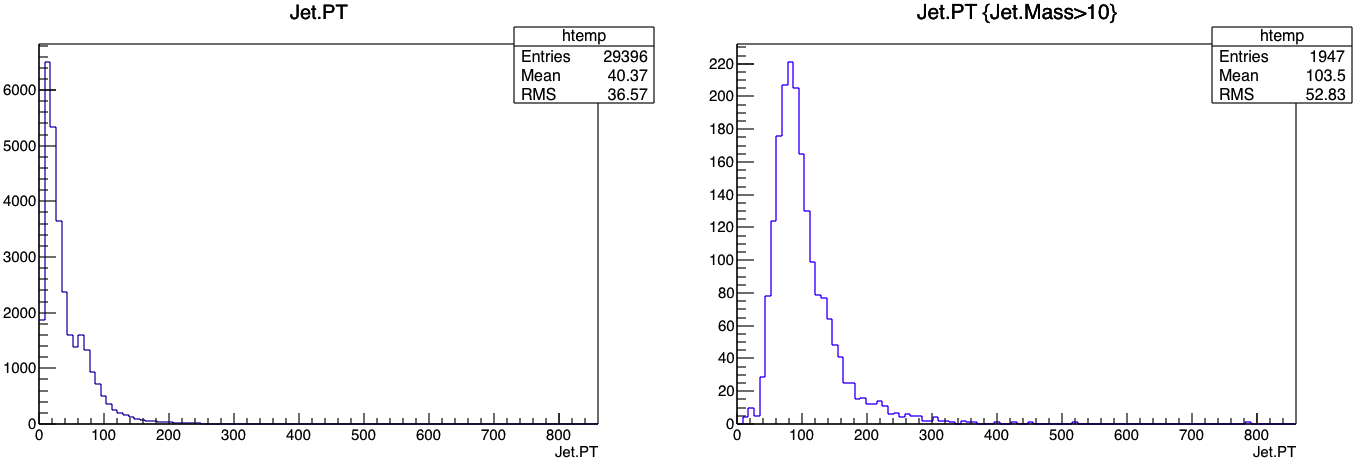
\includegraphics[width=\textwidth]{figures/JetPT.png}
\caption{The number of entries versus the transverse momentum of the leading jet using 50,000 $\Pp\Pp \rightarrow \Ppositron \Pelectron$ events simulated in \madgraph. The left panel shows the raw histogram and the right shows the effect of adding a cut on the mass of the jet $>10\GeV$.}
\end{figure}

\begin{figure}[htbp]
\centering
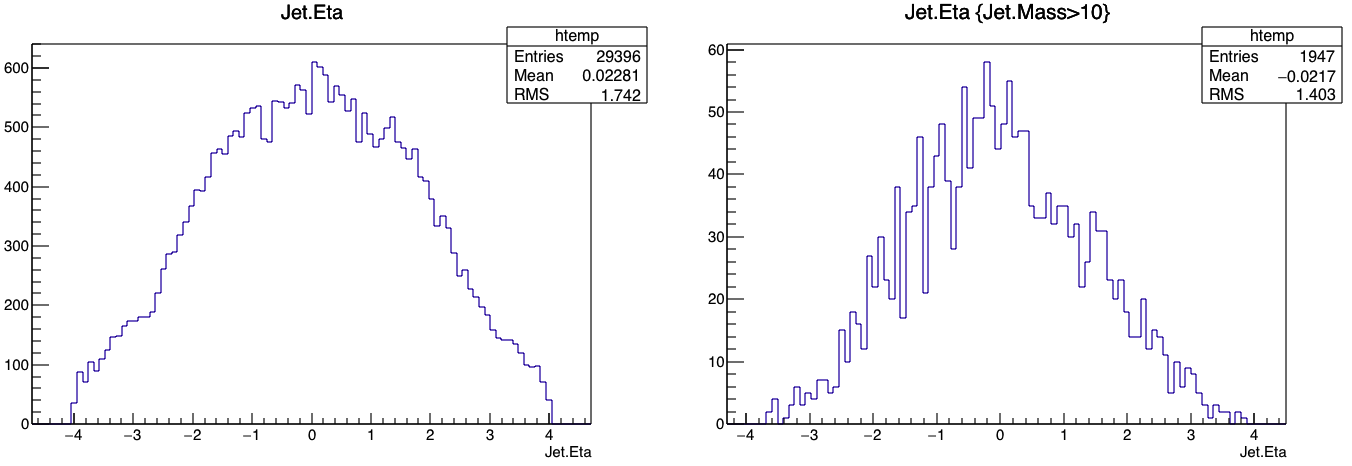
\includegraphics[width=\textwidth]{figures/JetEta.png}
\caption{The number of entries versus the pseudorapidity of the leading jet using 50,000 $\Pp\Pp \rightarrow \Ppositron \Pelectron$ events simulated in \madgraph. The left panel shows the raw histogram and the right shows the effect of adding a cut on the mass of the jet $>10\GeV$.}
\end{figure}

\begin{figure}[htbp]
\centering
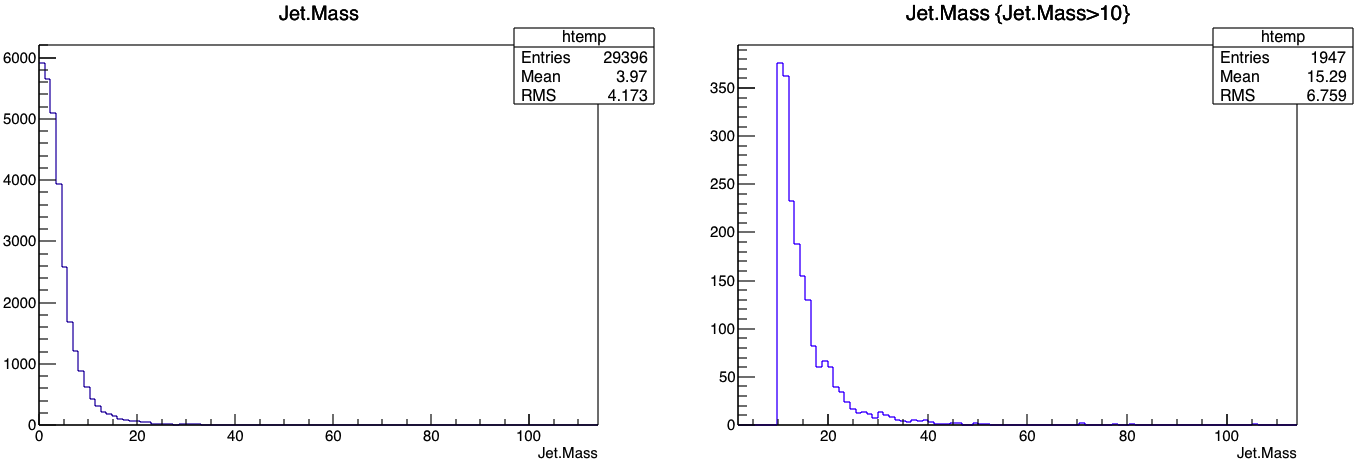
\includegraphics[width=\textwidth]{figures/JetMass.png}
\caption{The number of entries versus the mass of the leading jet using 50,000 $\Pp\Pp \rightarrow \Ppositron \Pelectron$ events simulated in \madgraph. The left panel shows the raw histogram and the right shows the effect of adding a cut on the mass of the jet $>10\GeV$.}
\end{figure}

\begin{figure}[htbp]
\centering
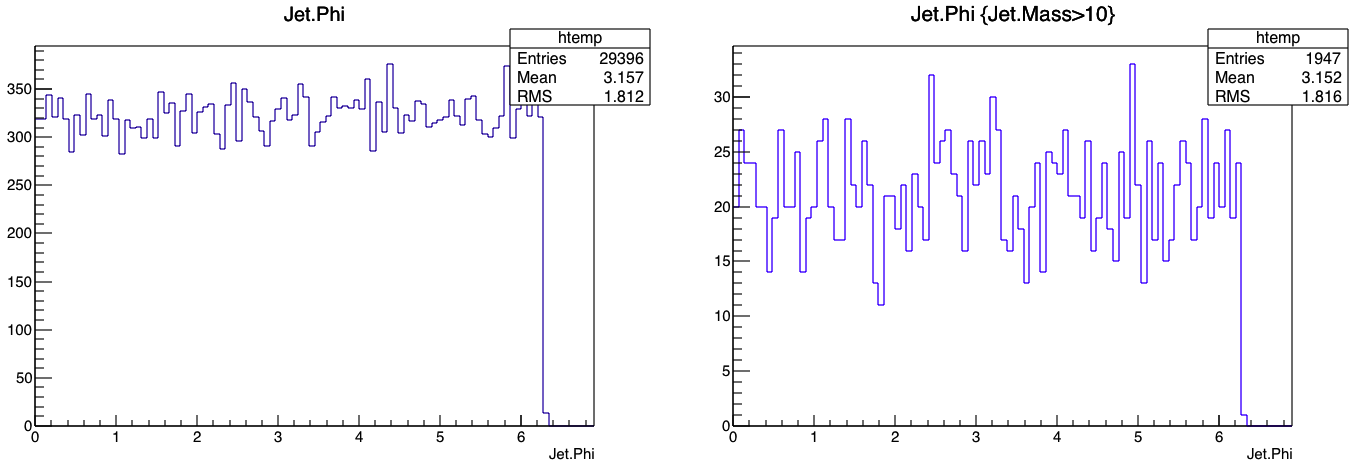
\includegraphics[width=\textwidth]{figures/JetPhi.png}
\caption{The number of entries versus the phi (meaning?) of the leading jet using 50,000 $\Pp\Pp \rightarrow \Ppositron \Pelectron$ events simulated in \madgraph. The left panel shows the raw histogram and the right shows the effect of adding a cut on the mass of the jet $>10\GeV$.}
\end{figure}

It is obvious that even with a small cut on jet mass, the histograms noticeably change. For the jet mass plot, it retains the same shape after the cut because were effectively only changing the range. But applying a cut on jet mass excludes different relevant data for jet $\phi$, jet $\eta$, jet \pt, etc. so the plots look quite different. This kind of analysis can be used to determine the dependencies of certain variables on others, e.g., when you change/exclude certain ranges of jet \pt, how does the histogram for jet mass change? And so on. This will be especially useful when analysing real LHC data to try and determine, not just the mass, but different properties of dark matter and different particle decay modes.

I've also figured out how to plot a histogram, and then overlay the histogram after a cut on the same axes. I've also streamlined my Python script readjets.py by storing the variable names and the cuts as character strings. So if I want to change the cut or change one of the variables I want to look at, I only have to edit part of one line as opposed to multiple entries throughout the script. An example plot and the new script are displayed below.

\begin{figure}[htbp]
\centering
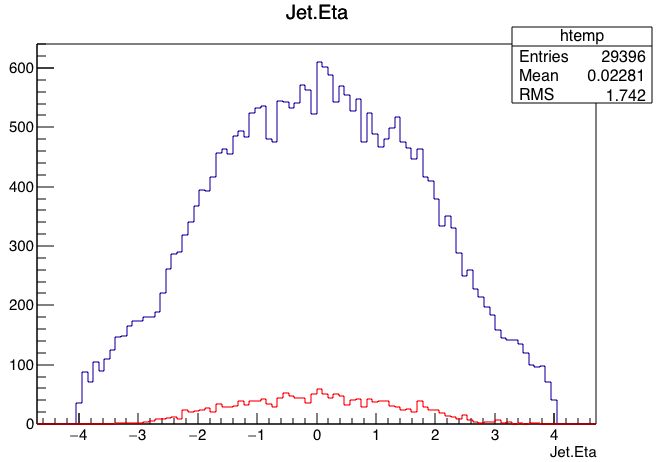
\includegraphics[width=\textwidth]{figures/JetEtalargecut.png}
\caption{The number of entries versus the pseudorapidity of the leading jet using 50,000 $\Pp\Pp \rightarrow \Ppositron \Pelectron$ events simulated in \madgraph. The blue line shows the raw data and the red line shows the effect of a cut on jet $\pt > 100\GeV$.}
\end{figure}

\lstinputlisting[language=Python, caption={A Python script used to print histograms with a cut on the same axes. File name: readjets.py (v2).}]{listings/readjetsv2.py}
